\documentclass{amsart}
\usepackage{amsmath}
\usepackage{amssymb}
\usepackage{amsthm}
%\usepackage{MnSymbol}
\usepackage{bm}
\usepackage{accents}
\usepackage{mathtools}
\usepackage{tikz}
\usetikzlibrary{calc}
\usetikzlibrary{decorations.pathmorphing,shapes}
\usetikzlibrary{automata,positioning}
\usepackage{tikz-cd}
\usepackage{forest}
\usepackage{braket} 
\usepackage{listings}
\usepackage{mdframed}
\usepackage{verbatim}
\usepackage{physics}
\usepackage{stmaryrd}
\usepackage{mathrsfs} 
\usepackage{stackengine} 
%\usepackage{/home/patrickl/homework/macaulay2}

%font
\usepackage[osf]{mathpazo}
\usepackage{microtype}

%CS packages
\usepackage{algorithmicx}
\usepackage{algpseudocode}
\usepackage{algorithm}

% typeset and bib
\usepackage[english]{babel} 
\usepackage[utf8]{inputenc} 
%\usepackage[backend=biber, style=alphabetic]{biblatex}
\usepackage[bookmarks, colorlinks, breaklinks]{hyperref} 
\hypersetup{linkcolor=black,citecolor=black,filecolor=black,urlcolor=black}

% other formatting packages
\usepackage{float}
\usepackage{booktabs}
\usepackage[shortlabels]{enumitem}
\usepackage{csquotes}
%\usepackage{titlesec}
%\usepackage{titling}
%\usepackage{fancyhdr}
%\usepackage{lastpage}
\usepackage{parskip}

\usepackage{lipsum}

% delimiters
\DeclarePairedDelimiter{\gen}{\langle}{\rangle}
\DeclarePairedDelimiter{\floor}{\lfloor}{\rfloor}
\DeclarePairedDelimiter{\ceil}{\lceil}{\rceil}


\newtheorem{thm}{Theorem}[section]
\newtheorem{cor}[thm]{Corollary}
\newtheorem{prop}[thm]{Proposition}
\newtheorem{lem}[thm]{Lemma}
\newtheorem{conj}[thm]{Conjecture}
\newtheorem{quest}[thm]{Question}

\theoremstyle{definition}
\newtheorem{defn}[thm]{Definition}
\newtheorem{defns}[thm]{Definitions}
\newtheorem{con}[thm]{Construction}
\newtheorem{exm}[thm]{Example}
\newtheorem{exms}[thm]{Examples}
\newtheorem{notn}[thm]{Notation}
\newtheorem{notns}[thm]{Notations}
\newtheorem{addm}[thm]{Addendum}
\newtheorem{exer}[thm]{Exercise}

\theoremstyle{remark}
\newtheorem{rmk}[thm]{Remark}
\newtheorem{rmks}[thm]{Remarks}
\newtheorem{warn}[thm]{Warning}
\newtheorem{sch}[thm]{Scholium}


% unnumbered theorems
\theoremstyle{plain}
\newtheorem*{thm*}{Theorem}
\newtheorem*{prop*}{Proposition}
\newtheorem*{lem*}{Lemma}
\newtheorem*{cor*}{Corollary}
\newtheorem*{conj*}{Conjecture}

% unnumbered definitions
\theoremstyle{definition}
\newtheorem*{defn*}{Definition}
\newtheorem*{exer*}{Exercise}
\newtheorem*{defns*}{Definitions}
\newtheorem*{con*}{Construction}
\newtheorem*{exm*}{Example}
\newtheorem*{exms*}{Examples}
\newtheorem*{notn*}{Notation}
\newtheorem*{notns*}{Notations}
\newtheorem*{addm*}{Addendum}


\theoremstyle{remark}
\newtheorem*{rmk*}{Remark}

% shortcuts
\newcommand{\Ima}{\mathrm{Im}}
\newcommand{\A}{\mathbb{A}}
\newcommand{\G}{\mathbb{G}}
\newcommand{\N}{\mathbb{N}}
\newcommand{\R}{\mathbb{R}}
\newcommand{\C}{\mathbb{C}}
\newcommand{\Z}{\mathbb{Z}}
\newcommand{\Q}{\mathbb{Q}}
\renewcommand{\k}{\Bbbk}
\renewcommand{\P}{\mathbb{P}}
\newcommand{\M}{\overline{M}}
\newcommand{\g}{\mathfrak{g}}
\newcommand{\h}{\mathfrak{h}}
\newcommand{\n}{\mathfrak{n}}
\renewcommand{\b}{\mathfrak{b}}
\newcommand{\ep}{\varepsilon}
\newcommand*{\dt}[1]{%
   \accentset{\mbox{\Huge\bfseries .}}{#1}}
%\renewcommand{\abstractname}{Official Description}
\newcommand{\mc}[1]{\mathcal{#1}}
\newcommand{\msc}[1]{\mathscr{#1}}
\newcommand{\T}{\mathbb{T}}
\newcommand{\mf}[1]{\mathfrak{#1}}
\newcommand{\mr}[1]{\mathrm{#1}}
\newcommand{\ms}[1]{\mathsf{#1}}
\newcommand{\ol}[1]{\overline{#1}}
\newcommand{\ul}[1]{\underline{#1}}
\newcommand{\wt}[1]{\widetilde{#1}}
\newcommand{\wh}[1]{\widehat{#1}}
\renewcommand{\div}{\operatorname{div}}

\DeclareMathOperator{\Der}{Der}
\DeclareMathOperator{\Hom}{Hom}
\DeclareMathOperator{\End}{End}
\DeclareMathOperator{\ad}{ad}
\DeclareMathOperator{\Aut}{Aut}
\DeclareMathOperator{\Rad}{Rad}
\DeclareMathOperator{\Pic}{Pic}
\DeclareMathOperator{\supp}{supp}
\DeclareMathOperator{\sgn}{sgn}
\DeclareMathOperator{\spec}{Spec}
\DeclareMathOperator{\Spec}{Spec}
\DeclareMathOperator{\proj}{Proj}
\DeclareMathOperator{\Proj}{Proj}
\DeclareMathOperator{\ord}{ord}
\DeclareMathOperator{\Div}{Div}
\DeclareMathOperator{\Bl}{Bl}

\title{Fine moduli memes for $1$-categorical teens}
\author{Patrick Lei}
\date{April 2, 2021}

\begin{document}
    
\maketitle

\begin{abstract}
    We will discuss the moduli space of stable curves of genus $0$ with $n$ marked points and its intersection theory, following~\cite{keel}. We will give a nice presentation of its Chow ring in terms of boundary divisors.
\end{abstract}

\section{The moduli space}%
\label{sec:the_moduli_space}

The space $\ol{M}_{0,n}$ parameterizes curves that look like this:
\begin{figure}[H]
\begin{center}
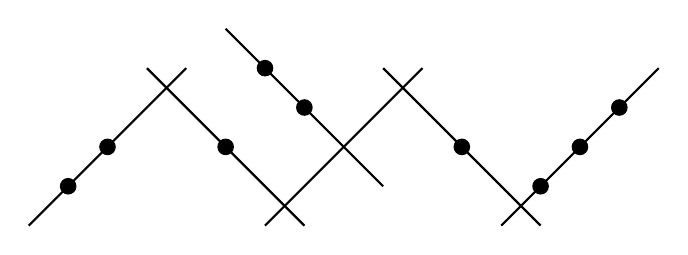
\begin{tikzpicture}[scale=1, transform shape]
    \draw[thick] (0,0) -- (2,2);
    \draw[thick] (1.5,2) -- (3.5,0);
    \draw[thick] (3,0) -- (5,2);
    \draw[thick] (4.5,2) -- (6.5,0);
    \draw[thick] (6,0) -- (8,2);
    \draw[thick] (2.5,2.5) -- (4.5,0.5);
    \fill (0.5,0.5) circle (3pt);
    \fill (1,1) circle (3pt);
    \fill (2.5,1) circle (3pt);
    \fill (3,2) circle (3pt);
    \fill (3.5,1.5) circle (3pt);
    \fill (5.5,1) circle (3pt);
    \fill (6.5,0.5) circle (3pt);
    \fill (7,1) circle (3pt);
    \fill (7.5,1.5) circle (3pt);
\end{tikzpicture}
\end{center}
\caption{A stable curve}%
\label{fig:stabcurve}
\end{figure}
More precisely, these are reduced connected curves that are a tree of $\P^1$s such that each $\P^1$ has at least three marked points or nodes. In addition, at most two components meet at each node and we want $H^1(C, \msc{O}_C) = 0$. If all of these conditions are satisfied, we call our curve \textit{stable}. More precisely, we want to represent the functor
\[ S \mapsto \left\{ 
\begin{tikzcd}
    \msc{C} \ar{r}{\pi} & S \ar[bend left=40]{l}{s_1, \ldots, s_n}   
\end{tikzcd} \text{ flat, proper } \Biggm\vert \Centerstack{ {$s_1, \ldots, s_n$ disjoint sections} {geometric fibers are stable curves} }
\right\}. \]

\begin{thm}[Knudsen]
    There exists a smooth complete variety $\ol{M}_{0,n}$ and universal curve $U_{0,n} \to \ol{M}_{0,n}$ with universal sections $s_1, \ldots, s_n$ that is a fine moduli space for this functor. $\ol{M}_{0,n}$ also contains the space $M_{0,n} = {(\P^1 \setminus \qty{0,1,\infty})}^{n-3} \setminus \Delta$ as a dense open subset.
\end{thm}

In fact, Knudsen also shows that $U_{0,n} = \ol{M}_{0, n+1}$ and $U_{0,n+1}$ is a blowup of $\ol{M}_{0,n+1} \times_{\ol{M}_{0,n}} \ol{M}_{0,n+1}$ along some subscheme of the diagonal. In order to prove this, Knudsen introduces two operations that we can perform, called contraction and stabilization. Contraction happens when we delete a marked point and stabilization happens when we add a marked point.

\begin{thm}[Knudsen]
    Contraction and stabilization are functorial! Moreover, they commute with base change.
\end{thm}
Here are some pictorial depictions of our operations:
\begin{figure}[H]
\begin{center}
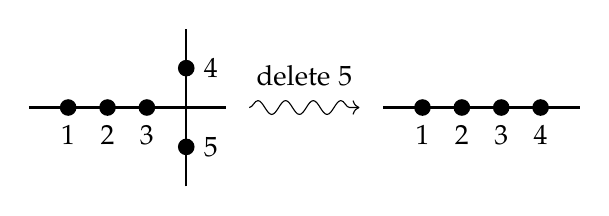
\begin{tikzpicture}[scale=1, transform shape]
    \draw[thick] (0,0) -- (2.5,0);
    \draw[thick] (2,-1) -- (2,1);
    \fill (0.5,0) circle (3pt);   
    \fill (1,0) circle (3pt);   
    \fill (1.5,0) circle (3pt);   
    \fill (2,-0.5) circle (3pt);
    \fill (2,0.5) circle (3pt);
    \node [right] at (2.1,0.5) {$4$};
    \node [right] at (2.1,-0.5) {$5$};
    \node [below] at (0.5,-0.1) {$1$};
    \node [below] at (1,-0.1) {$2$};
    \node [below] at (1.5,-0.1) {$3$};
    \node at (3.5,0.4) {delete $5$};
    \draw[->, decorate, decoration=snake] (2.8,0) -- (4.2,0);
    \draw[thick] (4.5,0) -- (7,0);
    \fill (5,0) circle (3pt);
    \fill (5.5,0) circle (3pt);
    \fill (6,0) circle (3pt);
    \fill (6.5,0) circle (3pt);
    \node [below] at (5,-0.1) {$1$};
    \node [below] at (5.5,-0.1) {$2$};
    \node [below] at (6,-0.1) {$3$};
    \node [below] at (6.5,-0.1) {$4$};
\end{tikzpicture}
\end{center}
\caption{Contraction}%
\label{fig:contract}
\end{figure}

\begin{figure}[htpb]
\begin{center}
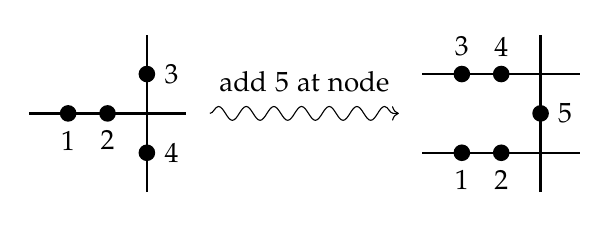
\begin{tikzpicture}[scale=1, transform shape]
    \draw[thick] (0,0) -- (2,0);
    \draw[thick] (1.5,-1) -- (1.5,1);
    \fill (0.5,0) circle (3pt);   
    \fill (1,0) circle (3pt);   
    \node [below] at (0.5,-0.1) {$1$};
    \node [below] at (1,-0.1) {$2$};
    \fill (1.5,-0.5) circle (3pt);
    \fill (1.5,0.5) circle (3pt);
    \node [right] at (1.6,0.5) {$3$};
    \node [right] at (1.6,-0.5) {$4$};
    \node at (3.5,0.4) {add $5$ at node};
    \draw[->, decorate, decoration=snake] (2.3,0) -- (4.7,0);
    \draw[thick] (5,-0.5) -- (7,-0.5);
    \draw[thick] (6.5,-1) -- (6.5,1);
    \draw[thick] (5,0.5) -- (7,0.5);
    \fill (5.5,-0.5) circle (3pt);
    \fill (6,-0.5) circle (3pt);
    \fill (5.5,0.5) circle (3pt);
    \fill (6,0.5) circle (3pt);
    \fill (6.5,0) circle (3pt);
    \node [below] at (5.5,-0.6) {$1$};
    \node [below] at (6,-0.6) {$2$};
    \node [above] at (5.5,0.6) {$3$};
    \node [above] at (6,0.6) {$4$};
    \node [right] at (6.6,0) {$5$};
\end{tikzpicture}
\end{center}
\caption{Stabilization (1)}%
\label{fig:stab1}
\end{figure}

\begin{figure}[H]
\begin{center}
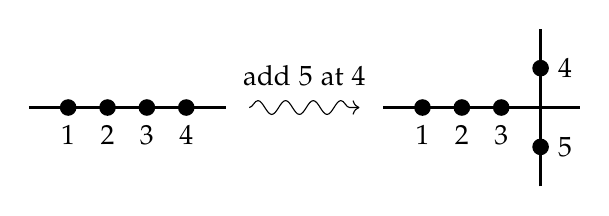
\begin{tikzpicture}[scale=1, transform shape]
    \draw[thick] (4.5,0) -- (7,0);
    \draw[thick] (6.5,-1) -- (6.5,1);
    \fill (5,0) circle (3pt);   
    \fill (5.5,0) circle (3pt);   
    \fill (6,0) circle (3pt);   
    \fill (6.5,-0.5) circle (3pt);
    \fill (6.5,0.5) circle (3pt);
    \node [right] at (6.6,0.5) {$4$};
    \node [right] at (6.6,-0.5) {$5$};
    \node [below] at (5,-0.1) {$1$};
    \node [below] at (5.5,-0.1) {$2$};
    \node [below] at (6,-0.1) {$3$};
    \node at (3.5,0.4) {add $5$ at $4$};
    \draw[->, decorate, decoration=snake] (2.8,0) -- (4.2,0);
    \draw[thick] (0,0) -- (2.5,0);
    \fill (0.5,0) circle (3pt);
    \fill (1,0) circle (3pt);
    \fill (1.5,0) circle (3pt);
    \fill (2,0) circle (3pt);
    \node [below] at (0.5,-0.1) {$1$};
    \node [below] at (1,-0.1) {$2$};
    \node [below] at (1.5,-0.1) {$3$};
    \node [below] at (2,-0.1) {$4$};
\end{tikzpicture}
\end{center}
\caption{Stabilization (2)}%
\label{fig:stab2}
\end{figure}

\section{Keel construction of $\ol{M}_{0,n}$}%
\label{sec:keel_construction_of_m__0_n_}

First, we will describe the boundary divisors of $\ol{M}_{0,n}$. Let $T \subseteq \qty{1,\ldots, n} \eqqcolon [n]$ satisfy $\abs{T}, \abs{T^C} \geq 2$. Then define 
\[ D^T \coloneqq \overline{ \left\{ 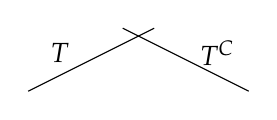
\begin{tikzpicture}[scale=0.8]
    \draw (0,-0.5) -- (2,0.5);
    \draw (1.5,0.5) -- (3.5,-0.5);
    \node at (0.5,0.1) {$T$};
    \node at (3,0.1) {$T^C$};
\end{tikzpicture} \right\} }. \]
It is easy to see that $D^T = D^{(T^C)}$. Knudsen proves that $D^T$ is a smooth divisor and that $D^T \cong \ol{M}_{\abs{T}+1} \times \ol{M}_{\abs{T^C}+1}$.

Now consider the map $\pi \colon \ol{M}_{0,n+1} \to \ol{M}_{0,n}$ coming from the identification $\ol{M}_{0, n+1} = U_{0, n}$. Now Keel proves that we can factor $\pi$ as
\[ \ol{M}_{0,n+1} \xrightarrow{\pi_1 = (\pi, \pi_{1,2,3,n+1})} \ol{M}_{0,n} \times \ol{M}_{0,4} \xrightarrow{p_1} \ol{M}_{0,n}, \]
where $\pi_{1,2,3,n+1} \colon \ol{M}_{0,n+1} \to \ol{M}_{0,n}$ forgets all sections besides $1,2,3,n+1$. Next, Keel shows that $\pi_1$ is a composition of blowups along smooth codimension $2$ subvarieties using an inductive construction.

Set $B_1 = \ol{M}_{0,n} \times \ol{M}_{0,4}$. Then the universal sections $s_1, \ldots, s_n \colon \ol{M}_{0,n} \to \ol{M}_{0,n+1}$ induce sections $p \circ s_1, \ldots, p \circ s_n$. In fact, $D^T \cong p \circ s_i(D^T)$ and this is independent of $i$. We also have

\begin{lem}[Keel]
    The divisors $D^T \subset \ol{M}_{0,n+1}$ with $T \subset [n]$ are the exceptional divisors of $\pi_1$.
\end{lem}

Now we set $B_2$ to be the blowup of $B_1$ at $\bigcup_{\abs{T^C}=2} D^T$. Inductively, we set $B_{k+1}$ to be the blowup of $B_k$ at $\bigcup_{\abs{T^C}=k+1} D^T$. Now we summarize the main results as follows:

\begin{thm}[Keel]
    The map $\pi_1$ factors through $B_k$ and $\ol{M}_{0,n+1} = B_{n-2}$.
\end{thm}

\section{Intersection theory of $\ol{M}_{0,n}$}%
\label{sec:intersection_theory_of_m__0_n_}

There are several major results about the intersection theory of $\ol{M}_{0,n}$. In fact, once we state these results, we will only be seven pages through Keel's paper, and the rest of the paper is dedicated to proving these results.

\begin{thm}
    We have an isomorphism $A_*(\ol{M}_{0,n}) \to H_*(\ol{M}_{0,n})$. In particular, $\ol{M}_{0,n}$ has no odd homology and $A_*(\ol{M}_{0,n+1})$ is a finitely generated free abelian group. In fact, if a scheme $Y$ satisfies $A^*(Y) = H^*(Y)$, then so does $Y \times \ol{M}_{0,n}$.
\end{thm}

\begin{thm}
    For any scheme $S$, there is an isomorphism $A^*(\ol{M}_{0,n} \times S) = A^*(\ol{M}_{0,n}) \otimes A^*(S)$.
\end{thm}

\begin{thm}
    For all $k$, we have an isomorphism
    \[ A^k(\ol{M}_{0,n+1}) \cong A^k(\ol{M}_{0,n}) \oplus A^{k-1}(\ol{M}_{0,n}) \oplus \bigoplus_{\substack{T \subset [n] \\ \abs{T \cap [3]} \leq 1}} A^{k-1}(D^T) \]
    which is induced by the maps
    \begin{align*}
        A^k(\ol{M}_{0,n}) \xrightarrow{\pi^*} A^k(\ol{M}_{0,n+1}) \\
        A^{k-1}(\ol{M}_{0,n}) \xrightarrow{\pi^*} A^{k-1}(\ol{M}_{0,n+1}) \xrightarrow{\cup \pi_{1,2,3,n+1}^* (c_1(\msc{O}(1)))} A^k(\ol{M}_{0,n+1}) \\
        A^{k-1}(D^T) \xrightarrow{g^*} A^{k-1}(D^{T \subset [n+1]}) \xrightarrow{j_*} A^k(\ol{M}_{0,n+1}),
    \end{align*}
    where $g,j$ are as in the diagram
    \begin{equation*}
    \begin{tikzcd}
        D^{T \subset [n+1]} \ar{d}{g} \ar[hookrightarrow]{r}{j} & \ol{M}_{0,n+1} \ar{d}{\pi} \\
        D^T \ar[hookrightarrow]{r}{i} & \ol{M}_{0,n}.
    \end{tikzcd}
    \end{equation*}
\end{thm}

\begin{thm}
    The Chow groups $A^k(\ol{M}_{0,n})$ are free abelian and the ranks $a^k(n) = \operatorname{rk}(A^k(\ol{M}_{0,n}))$ are given by the recursive formula
    \[ a^k(n+1) = a^k(n) + a^{k-1}(n) + \frac{1}{2} \sum_{j=2}^{n-2} \binom{n}{j} \sum_{\ell=0}^{k-1} a^{\ell}(j+1) a^{k-1-\ell}( n-j-1 ). \]
    In particular, we have the Picard rank $a^1(n) = 2^{n-1} - \binom{n}{2} - 1$.
\end{thm}

\begin{thm}
    The Chow ring $A^*(\ol{M}_{0,n})$ is the quotient of $\Z[D^T \mid T \subset [n], \abs{T}, \abs{T^C} \geq 2]$
    by the relations
    \begin{enumerate}
        \item $D^T = D^{(T^C)}$;
        \item For any distinct $i,j,k,\ell \in [n]$, we have the equality
            \[ \sum_{\substack{i.j\in T \\ k,\ell \notin T}} D^T = \sum_{\substack{i,k\in T \\ j,\ell \notin T}} D^T = \sum_{\substack{i,\ell \in T \\ j,k \notin T}} D^T. \]
        \item For $T_1, T_2 \subset [n]$, $D^{T_1} D^{T_2} = 0$ unless one of $T_1 \subset T_2, T_2 \subset T_1, T_1 \subset T_2^C, T_2 \subset T_1^C$ holds.
    \end{enumerate}
\end{thm}

\begin{rmk}
    All of the relations encode geometric content:
    \begin{enumerate}
        \item As divisors, we already know that $D^T = D^{(T^C)}$.
        \item If we consider the map $\pi_{i,j,k,\ell} \colon \ol{M}_{0,n} \to \M_{0,4}$, then the three sums are the pullbacks of the three boundary divisors $D^{i,j}, D^{i,k}, D^{i,\ell} \subset \M_{0,4} = \P^1$.
        \item The final relation encodes the fact that $D^{T_1} \cap D^{T_2} = \emptyset$ unless one of the four inclusions holds. Pictorially, this is encoded in the diagram below:
            \begin{figure}[htpb]
            \begin{center}
            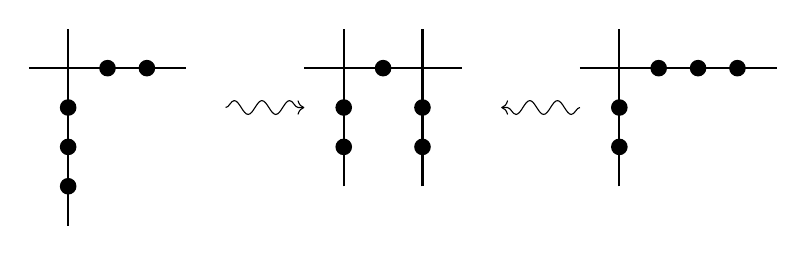
\begin{tikzpicture}[scale=1, transform shape]
                \draw[thick] (0,-0.5) -- (0,2);
                \draw[thick] (-0.5,1.5) -- (1.5,1.5);
                \fill (0,0.5) circle (3pt);
                \fill (0,1) circle (3pt);
                \fill (0,0) circle (3pt);
                \fill (0.5,1.5) circle (3pt);
                \fill (1,1.5) circle (3pt);
                \draw[->, decorate, decoration=snake] (2,1) -- (3,1);
                \draw[thick] (3.5,0) -- (3.5,2);
                \draw[thick] (3,1.5) -- (5,1.5);
                \draw[thick] (4.5,0) -- (4.5,2);
                \fill (3.5,0.5) circle (3pt);
                \fill (3.5,1) circle (3pt);
                \fill (4,1.5) circle (3pt);
                \fill (4.5,0.5) circle (3pt);
                \fill (4.5,1) circle (3pt);
                \draw[->, decorate, decoration=snake] (6.5,1) -- (5.5,1);
                \draw[thick] (7,0) -- (7,2);
                \draw[thick] (6.5,1.5) -- (9,1.5);
                \fill (7,0.5) circle (3pt);
                \fill (7,1) circle (3pt);
                \fill (7.5,1.5) circle (3pt);
                \fill (8, 1.5) circle (3pt);
                \fill (8.5,1.5) circle (3pt);
            \end{tikzpicture}
            \end{center}
            \caption{Degeneration to a common stable curve}%
            \label{fig:degen}
            \end{figure}
    \end{enumerate}
\end{rmk}

\section{Intersection theory of regular blowups}%
\label{sec:intersection_theory_of_regular_blowups}

Let $i \colon X \subset Y$ be a regularly embedded subvariety, $\pi \colon \wt{Y} \to Y$ be the blowup along $X$, and $\wt{X}$ be the exceptional divisor. Let $g \colon \wt{X} \to X$ and $j \colon \wt{X} \to \wt{Y}$.

\begin{thm}
    Suppose $i^*$ is surjective. Then
    \[ A^*(\wt{Y}) = \frac{A^*(Y)[T]}{(P(T), T \cdot \ker(i^*))}, \]
    where $P(T)$ has constant term $[X]$ and $i^* P(T) = T^d + T^{d-1} c_1(N_X Y) + \cdots + c_d(N_X Y)$, where $d$ is the codimension of $X$ in $Y$. This is induced by $-T = [\wt{X}]$.
\end{thm}

\begin{thm}
    A scheme $X$ is HI if $A_*(X) = H_*(X)$. If $X, Y$ are both HI, then so is $\wt{Y}$.
\end{thm}

\begin{thm}
    The map
    \[ A_k(Y) \oplus A_{k-1}(X) \xrightarrow{(\pi^*, j_* g^*)} A_k(\wt{Y}) \]
    is an isomorphism.
\end{thm}

\begin{thebibliography}{9}
    \bibitem{keel} Sean Keel, \textit{Intersection theory of moduli space of stable N-pointed curves of genus zero}, Transactions of the American Mathematical Society, Vol. 300, No. 2 (April 1992), pp. 545-574. 
\end{thebibliography}




\end{document}
